% !TeX encoding = UTF-8
% !TeX spellcheck = sk_SK
\documentclass[]{tukediphc}
%% -----------------------------------------------------------------
%% tento subor ma kodovanie utf-8
%%
%% na kompilaciu pouzivajte format pdflatex 
%%
%% V pripade problemov kontaktujte Jána Bušu st. (jan.busa@tuke.sk)
%%
%% November 2015
%% -----------------------------------------------------------------
%%
%\usepackage[dvips]{graphicx}
%\DeclareGraphicsExtensions{.eps}
\usepackage[pdftex]{graphicx}
\usepackage{ragged2e}
\usepackage{pdfpages}


\DeclareGraphicsExtensions{.pdf,.png,.jpg,.mps,.svg}
\graphicspath{{figures/}} % priecinok na obrazky
%%


%\usepackage[utf8]{inputenc}  % je v cls-subore
%\usepackage[T1]{fontenc}  % je v cls-subore
\usepackage{lmodern,textcase}
\usepackage[slovak]{babel}
\def\refname{Zoznam použitej literatúry}
\usepackage{latexsym}
\usepackage{dcolumn} % zarovnanie cisiel v tabulke podla des. ciarky
\usepackage{hhline}
\usepackage{amsmath,amsfonts,amssymb}

\usepackage{indentfirst}
\usepackage{parskip}
\setlength{\parskip}{1em}

\usepackage{nicefrac} % pekne zlomky
\usepackage{upgreek} % napr. $\upmu\mathrm{m}$ pre mikrometer ...
\usepackage[final]{showkeys}%color%notref%notcite%final
\usepackage[slovak,noprefix]{nomencl}

\makeglossary % prikaz na vytvorenie suboru .glo


% Pouzit v pripade velkeho poctu subsection v tableofcontents
% \makeatletter
% \renewcommand*\l@subsection{\@dottedtocline{2}{1.5em}{3.5em}}
% \newcommand*\l@subsection{\@dottedtocline{2}{1.5em}{2.3em}}
% \newcommand*\l@subsubsection{\@dottedtocline{3}{3.8em}{3.2em}}
% \makeatother


%\def\thefigure{\Roman{section}.\arabic{figure}}

%\usepackage{parskip}% 'zhusti' polozky obsahu
%% Cislovane citovanie
\usepackage[numbers]{natbib}

%%
%% Citovanie podľa mena autora a roku
%\usepackage{natbib} \citestyle{chicago}
% -----------------------------------------------------------------
%% tlač !!!
\usepackage[pdftex,unicode=true,bookmarksnumbered=true,
bookmarksopen=true,pdfmenubar=true,pdfview=Fit,linktocpage=true,
pageanchor=true,bookmarkstype=toc,pdfpagemode=UseOutlines,
pdfstartpage=1]{hyperref}
\hypersetup{%
baseurl={http://www.tuke.sk/sevcovic},
pdfcreator={pdfcsLaTeX},
pdfkeywords={Multi-robot navigation, target tracking, hunt-ing behavior, cooperative collision avoidance},
pdftitle={Využitie prostriedkov internetu vozidiel v navigácii mobilných robotov},
pdfauthor={Bohdan Tanasov},
pdfsubject={Diplomová práca}
} 
%% nehodiace zakomentujte !
\dippraca{Diplomová práca}
%\bakpraca{Bakalárska práca}
%%
\nazov{Využitie prostriedkov internetu vozidiel v navigácii mobilných robotov}
%% ked praca nema 'podnazov' zakomentujte nasledujuci riadok
%% alebo polozku nechajte prazdnu
\podnazov{}
\jazyk{Slovenský}
% anglicky nazov
\title{Simulation of Cooperation for a Multi-Robotic System}
\autor{Bohdan Tanasov}
\veduciprace{doc. Dr. Ing.~Ján~Vaščák}
\konzultanta{ing.~Dušan~Herich}
% \konzultantb{RNDr.~Marián~Čierny, DrSc.}
\titul{Bc}
\univerzita{Technická univerzita v~Košiciach}
\fakulta{Fakulta elektrotechniky a informatiky}
\skratkafakulty{FEI}
\katedra{Katedra umelej inteligencie}
\skratkakatedry{KUI}
\odbor{Informatika}
\specializacia{Inteligentné systémy}
\abstrakt{Cieľom tejto práce bolo vyvinúť automatizovaný systém riadenia pre bezpilotné lietadlo, ktorý využíva zabudovanú kameru na navigáciu a zber údajov. Systém bol implementovaný pomocou programovacieho jazyka Python spolu s balíkom OpenCV pre algoritmy počítačového videnia a značkami ArUco pre merania, NodeJS a React. 
Pomocou systému môžeme manipulovať s viacerými dronmi a so samostatným dronom z webovej stránky a môžeme vidieť údaje dronov a súradnice dronov v priestore pomocou značiek aruco.
Na záver možno konštatovať, že systém úspešne dosiahol svoj cieľ, ktorým je adaptácia autonómneho navigačného systému pre bezpilotné lietadlá v interiéri. Následne spracované súbory údajov boli dostatočne dobre filtrované, aby sa mohli považovať za adekvátne merania. Program by sa mohol v budúcnosti vylepšiť tak, aby podporoval viac príkazov pre skupiny dronov, napr. postaviť kolo alebo iné postavy. Takýto systém sa dá použiť aj pre priemyselné bezpilotné lietadlá, kde sú polohy AR markerov vopred známe.}
\abstrakte{The objective of this work was to develop an automated control system for an unmanned aircraft that uses an embedded camera for navigation and data collection. The system was implemented using the Python programming language along with the OpenCV package for computer vision algorithms and the ArUco tags for measurements, NodeJS and React. 
Using the system, we can manipulate multiple drones and a single drone from a web page and can see the drone data and drone coordinates in space using aruco tags.
In conclusion, the system has successfully achieved its goal of adapting an autonomous navigation system for drones indoors. The subsequently processed datasets were sufficiently well filtered to be considered as adequate measurements. The program could be improved in the future to support more commands for groups of drones, e.g., build a bike or other figures. Such a system could also be used for industrial drones where the positions of the AR markers are known in advance.}
\keywords{UAV, autonomous navigation, AR marker, positioning, measurements}
\klucoveslova{UAV, autonómna navigácia, AR marker, určovanie polohy, merania}

\datumodovzdania{21.~4.~2023}
\datumobhajoby{20.~5.~2023}
\mesto{Košice}
\pocetstran{\pageref{page:posledna}}
\kategoria{Záverečná práca} 

\begin{document}
\renewcommand{\figurename}{Obrázok}	
\renewcommand\theHfigure{\theHsection.\arabic{figure}}
\renewcommand\theHtable{\theHsection.\arabic{table}}

\prvastrana

\titulnastrana 

%\analytickylist


%\errata % zaciatok erraty
%Ak je potrebné, autor na tomto mieste opraví chyby, ktoré našiel po
%vytlačení práce. Opravy sa uvádzajú takým písmom, akým je napísaná
%práca. Ak zistíme chyby až po vytlačení a zviazaní práce, napíšem
%erráta na samostatný lístok, ktorý vložíme na toto miesto. Najlepšie je
%lístok prilepiť \citep{kat}.
%
%Forma:
%
%%\tabcolsep=10pt
%\begin{table}[!hb]
%	\centering
%	\begin{tabular}{|c|c|c|c|}\hline
%Strana & Riadok & Chybne & Správne \\\hline\hline
%12 & 6 & publikácia & prezentácia \\\hline
%22 & 23 & internet & intranet \\\hline
%& & & \\\hline
%& & & \\\hline
%	\end{tabular}
%\end{table}
%\kerrata % koniec erraty

\abstraktsk % abstrakt v SK 

\abstrakteng % abstrakt v ENG

\kabstrakt % koniec abstraktov, nova strana

% Na tomto mieste bude vložené zadanie diplomovej práce
% \zadanieprace{}
\includepdf[pages=-]{zadavaci-list.pdf}

\cestnevyhlasenie
% Niektorí autori metodických príručiek o~záverečných prácach sa
% nazdávajú, že takéto vyhlásenie je zbytočné, nakoľko povinnosť
% vypracovať záverečnú prácu samostatne, vyplýva študentovi zo zákona a
% na autora práce sa vzťahuje autorský zákon.

\podakovanie
Najskôr by som sa chcel poďakovať vedúcemu bakalárskej práce doc. Dr. Ing. Jánovi Vaščakovi. Príležitosť komunikovať s docentom Vaščakom bola vždy otvorená, kedykoľvek som narazil na problémové miesto alebo mal otázku o svojom výskume alebo písaní. Dôsledne pripúšťal, aby tato práca bola mojou vlastnou, ale vždy, keď si myslel, že to potrebujem, ma nasmeroval správnym smerom.

Na záver musím svojim rodičom poďakovať za to, že mi počas rokov štúdia a pri výskume a písaní tejto práce poskytovali neutíchajúcu podporu a neustále povzbudzovanie. Bez nich by tento úspech nebol možný. Ďakujem.
\kpodakovania

\predhovor
Téma práce sa zaoberá využitím dronov Tello v skupinovej koordinovanej misii, kde bola navrhnutá a implementovaná webová aplikácia, ktorá umožňuje ovládanie viacerých dronov naraz. V práci je tiež popísaná implementácia systému, ktorý umožňuje sledovanie pozície dronov pomocou kamery a detekcie Aruco markerov.
Cieľom tejto práce bolo ukázať, ako efektívne ovládať viacero dronov naraz pomocou jednoduchej webovej aplikácie a koordinovaného systému detekcie pozície dronov. V práci sa tiež zaoberáme riešeniami problémov pri použití viacerých dronov naraz a analyzujeme výsledky našich experimentov a testov.
% Zvýšil sa záujem o výskum v systémoch zložených z viacerých autonómnych mobilných robotov vykazujúcich kooperatívne správanie. Konštruujú sa skupiny mobilných robotov s cieľom študovať také problémy, ako je skupinová architektúra, konflikt zdrojov, pôvod spolupráce, učenie sa a geometrické problémy. Doposiaľ bolo opísaných málo aplikácií kooperatívnej robotiky a teória podpory je stále v štádiu formovania. V tejto prace bol vytvorený multi-robotický projekt a diskutované problémy a variácie ich riešenia 
\kpredhovoru

\thispagestyle{empty}
\tableofcontents
\thispagestyle{empty}

\newpage

\thispagestyle{empty}

{	\makeatletter
	\renewcommand{\l@figure}{\@dottedtocline{1}{1.5em}{3.5em}}
	\makeatother
	\listoffigures}

%\addcontentsline{toc}{section}{\numberline{}Zoznam obrázkov}
%\listoffigures


\newpage

\thispagestyle{empty}
%\addcontentsline{toc}{section}{\numberline{}Zoznam tabuliek}
\listoftables

\thispagestyle{empty}
\newpage
 
\thispagestyle{empty}
%\addcontentsline{toc}{section}{\numberline{}Zoznam symbolov a
%skratiek}
\printglossary % vlozenie zoznamu skratiek a symbolov
\newpage

%\addcontentsline{toc}{section}{\numberline{}Slovník termínov}
\slovnikterminov

\begin{description}
	\item[Virtuálna štruktúra] je štruktúra tvorená a udržiavaná skupinou robotov, ktorí prenasledujú cieľ
	\item[\boldmath $R_p$] je zápis na diagramoch a obrázkoch robota Korisť
	\item[\boldmath $R_1, R_2, R_3$] je záznam o schémach a obrázkoch robotov zo skupiny prenasledovateľov
	\item[ROS] Robot Operating System.
	\item[Robot Korisť] je robot, ktorým ovláda človek pomocou klávesnice a jeho cieľom je utekať pred skupinou prenasledovateľov.	\item[Robot Prenasledovateľ] je hlavný robot zo skupiny prenasledovateľov.
	\item[r] konštantná minimálna vzdialenosť, na ktorú sa robot Prenasledovateľ nesmie priblížiť ku robotovi Korisť.
	\item[d(P,A)] je vzdialenosť od robota prenasledovateľa k robotovi koristi v konkrétnom čase.
	\item[R] je určitá konštantná bezpečná vzdialenosť od robota Korisť po robota Prenasledovateľ, ktorú sa skupina prenasledovateľov snaží udržať v sledovacom režime
	\item[\boldmath$l_x$] je vzdialenosť. 
\end{description}

\kslovnikterminov
%
% !TeX encoding = UTF-8
% !TeX spellcheck = sk_SK
% !TeX root=tukedip.tex

\section*{Úvod}
\addcontentsline{toc}{section}{\numberline{}Úvod}
\setcounter{page}{1}
Drony sa v posledných rokoch stávajú čoraz populárnejšími vďaka svojej schopnosti vykonávať širokú škálu úloh, ktoré by inak boli pre človeka náročné alebo nebezpečné. Schopnosť ovládať viacero dronov súčasne otvára ešte viac možností ich využitia. Na dosiahnutie tohto cieľa je potrebné vyvinúť riadiaci systém, ktorý umožní efektívne a intuitívne ovládanie viacerých dronov. Cieľom tejto práce je vyvinúť takýto systém pomocou webovej aplikácie React a socketov.

Navrhovaný riadiaci systém umožní používateľovi ovládať viacero dronov Tello súčasne pomocou webového rozhrania. Použitie značiek Aruco umožní dronom zistiť ich polohu a podľa nej sa navigovať, čo umožní ovládať drony v individuálnom aj skupinovom režime. Systém bude pozostávať z backendu Node.js, ktorý bude zabezpečovať komunikáciu medzi webovou aplikáciou a dronmi, ako aj z programu Python bežiaceho na doske Asus TinkerBoard pripojenej ku každému dronu. Každý dron bude mať špecifické ID, čo umožní ich rozlíšenie.

Vývoj takéhoto riadiaceho systému predstavuje niekoľko výziev vrátane potreby zvládnuť komunikáciu v reálnom čase medzi dronmi a webovou aplikáciou, potreby presne zistiť polohu dronov a potreby zabezpečiť, aby sa systém ľahko používal a poskytoval dobrý používateľský zážitok.

Navrhovaný systém má potenciál na využitie v rôznych aplikáciách, ako je napríklad sledovanie pomocou dronov, letecké fotografovanie alebo pátracie a záchranné operácie. Tým, že systém umožňuje efektívne a intuitívne ovládanie viacerých dronov, by mohol pomôcť zvýšiť bezpečnosť a efektívnosť týchto operácií.

Zvyšok tejto práce je usporiadaný takto. V časti 2 sa uvádza prehľad príslušných technológií a metód, ktoré boli použité pri vývoji systému. V časti 3 je opísaný proces vývoja riadiaceho systému vrátane krokov vykonaných pri návrhu, implementácii a testovaní systému. V časti 4 sú uvedené výsledky práce vrátane podrobného opisu vyvinutého systému, jeho vlastností, používateľského rozhrania a funkčnosti, ako aj ukážky možností systému prostredníctvom príkladov použitia. V časti 5 sa hodnotí výkonnosť a použiteľnosť systému pomocou príslušných metrík a spätnej väzby od používateľov. Nakoniec sa v oddiele 6 uvádza zhrnutie výskumnej otázky, cieľov a prínosov, ako aj diskusia o obmedzeniach systému a možných cestách pre budúcu prácu a zlepšenie.
%
% !TeX encoding = UTF-8
% !TeX spellcheck = sk_SK
% !TeX root=tukedip.tex
\section{Formulácia úlohy}
\textbf{Analýza existujúcich prístupov a technológií pre využitie infraštruktúry internetu vozidiel v navigácii mobilných robotov.} 
Táto časť bakalárskej práce bude obsahovať analyz existujúcich prístupov a technológií pre využitie infraštruktúry internetu vozidiel v navigácii mobilných robotov. Tento bod sa bude venovať prehľadu existujúcich riešení a technológií, ktoré umožňujú mobilným robotom využívať internetové pripojenie vozidiel a ich infraštruktúru na navigáciu a pohyb.

\textbf{Návrh architektúry systému pre využitie prostriedkov internetu vozidiel v navigácii mobilných robotov.} 
V tejto časti sa budeme zaoberať návrhom architektúry systému pre využitie prostriedkov internetu vozidiel v navigácii mobilných robotov. V rámci tohto bodu sa bude riešiť návrh architektúry, ktorá umožní efektívne využívanie prostriedkov internetu vozidiel pre navigáciu mobilných robotov.

\textbf{Implementácia navrhnutého systému a jeho testovanie v rôznych prostrediach a scenároch.} 
Tato časť bude zahŕňať implementáciu navrhnutého systému a jeho testovanie v rôznych prostrediach a scenároch. Bude zahŕňať praktickú implementáciu navrhnutého systému a jeho otestovanie v rôznych reálnych prostrediach a podmienkach.

\textbf{Overenie funkčnosti a spoľahlivosti systému na lietajúcich vozidlách.} 
Táto kapitola sa bude zaoberať overením funkčnosti a spoľahlivosti systému na lietajúcich vozidlách. V rámci tohto bodu sa bude testovať funkčnosť a spoľahlivosť systému na lietajúcich vozidlách, aby sa zabezpečilo, že systém dokáže bezchybne fungovať aj v náročných podmienkach.

\textbf{Porovnanie výkonu a efektivity navrhnutého systému s existujúcimi prístupmia technológiami.} 
Tento bod sa bude zaoberať porovnaním výkonu a efektivity navrhnutého systému s existujúcimi prístupmi a technológiami. Tento bod bude zahŕňať porovnanie navrhnutého systému s existujúcimi riešeniami a technológiami, aby sa zistilo, ako dobre funguje navrhnutý systém v porovnaní s konkurenčnými riešeniami.

\textbf{Vypracovať dokumentáciu podľa pokynov vedúceho záverečnej práce.} 
Posledný bod sa bude zaoberať vypracovaním dokumentácie podľa pokynov vedúceho záverečnej práce. Tento bod bude zahŕňať vypracovanie dokumentácie, ktorá bude obsahovať kompletný popis navrhnutého systému, jeho implementáciu, testovanie a výsledky porovnania s existujúcimi riešeniami.

%
% !TeX root=tukedip.tex
% !TeX encoding = UTF-8
% !TeX spellcheck = sk_SK
\section{Prehľad literatúry}
Pred výberom metódy optického polohovania a navigácie sme museli preskúmať rôzne možnosti. Pozreli sme sa na metódy, ktoré by mohli byť vhodné na navigáciu dronov. Skúmala sa ich použiteľnosť pre mikrodrony.

\subsection{Optický princíp senzorov}
Snímače s optickým princípom sa bežne používajú v mobilnej robotike na navigáciu, lokalizáciu a mapovanie. Tieto senzory zachytávajú informácie z prostredia analýzou svetla a jeho interakcie s povrchmi, čím poskytujú bohaté údaje na presné určovanie polohy robota a plánovanie trajektórie. V tejto časti sa budeme zaoberať rôznymi typmi optických principiálnych snímačov a ich aplikáciami v mobilnej robotike \citep{Li2022}.

Jedným z najčastejšie používaných optických snímačov je kamera, ktorá zachytáva obrázky a videá prostredia. Kamery poskytujú bohaté vizuálne informácie vrátane farby, textúry a tvaru, ktoré možno využiť na detekciu, sledovanie a rozpoznávanie objektov. V našej práci využívame kamery namontované na bezpilotných lietadlách Tello na zisťovanie polohy značiek Aruco a odhadovanie ich súradníc v 3D priestore \citep{Li2022}. 

Ďalším dôležitým optickým senzorom je senzor LIDAR (Light Detection and Ranging), ktorý vysiela laserové lúče a meria ich odraz na vytvorenie 3D mapy prostredia. Senzory LIDAR sa bežne používajú v autonómnych vozidlách na vyhýbanie sa prekážkam a mapovanie. Sú však drahé a vyžadujú vysoký výpočtový výkon, čo ich robí menej vhodnými pre malú mobilnú robotiku \citep{Takahashi2014}.
 
Okrem kamier a LIDAR-u patria medzi ďalšie typy snímačov na optickom princípe infračervené snímače, ultrazvukové snímače a snímače času letu. Infračervené senzory merajú odraz infračerveného svetla na detekciu objektov a meranie ich vzdialenosti, zatiaľ čo ultrazvukové senzory vysielajú vysokofrekvenčné zvukové vlny a merajú ich ozvenu na odhad vzdialenosti. Snímače času letu využívajú svetlo na meranie času, za ktorý sa signál odrazí späť, čím poskytujú presné merania vzdialenosti.

Senzory na optickom princípe celkovo zohrávajú kľúčovú úlohu v mobilnej robotike a poskytujú bohaté informácie na navigáciu a lokalizáciu robota. Pochopením rôznych typov senzorov a ich aplikácií môžeme navrhnúť a implementovať efektívne robotické systémy, ktoré môžu fungovať v rôznych prostrediach a scenároch.

\subsection{Vyhýbanie sa prekážkam a orientácia na základe obrazu z kamery}
Jedným z najdôležitejších úloh mobilných robotov je schopnosť vyhnúť sa prekážkam a správne sa orientovať v prostredí. K dispozícii sú rôzne senzory, ktoré umožňujú robotom rozpoznať a vyhnúť sa prekážkam. Okrem senzorov ako LIDAR, ultrazvukových a infračervených senzorov sa dá využiť aj obraz z kamery.

Kamera poskytuje bohaté vizuálne informácie o prostredí a umožňuje robotom získavať informácie o prekážkach a teréne. Existujú rôzne spôsoby, ako využiť obraz z kamery pre navigáciu a vyhýbanie sa prekážkam.

\subsubsection{S vylepšenou neurónovou sieťou}
Jednou zo skúmaných metód na vyhýbanie sa prekážkam a orientáciu pomocou kamery bolo strojové učenie pomocou neurónových sietí. Nakoniec však bola zavrhnutá kvôli časovo a hardvérovo náročným procesom učenia. Táto metóda zahŕňa použitie naučenej neurónovej siete na priradenie približných hodnôt hĺbky každému pixelu na základe polohy objektov z jedného obrazu. Vzory sa dajú naučiť z dvojice LIDAR a digitálnych kamier umiestnených vedľa seba. Zadaním dostatočného počtu týchto naučených dvojíc môže neurónová sieť vytvoriť vzťah medzi pixelmi na obrázkoch a hodnotami hĺbky získanými z LIDAR-u alebo stereokamery.

Sieť sa môže učiť pomocou učenia založeného na LIDAR-e s dohľadom a učenia založeného na stereopároch bez dohľadu na základe pravdepodobnostného princípu. Učenie pod dohľadom je však často príliš prísne a učenie bez dohľadu poskytuje nepresné výsledky. Preto sa odporúča používať poloprevádzkové učenie alebo porovnávať výsledky získané pomocou siete s kalibrovaným systémom detekcie hĺbky počas prevádzky \citep{xie2016edge}.

Táto metóda získava hodnoty hĺbky z okolia a umiestnenia objektov (množiny pixelov) a vytvára mapu hĺbky podobnú tej, ktorá je znázornená na obrázku 1. Jej presnosť je zatiaľ experimentálna a takýto systém je stále vystavený mnohým chybám. Napriek tomu bol použitý v aplikáciách na riadenie dronov. Hĺbkové mapy na obrázku 1 ilustrujú rozdiel medzi rôznymi metódami a presnosť tejto metódy \citep{ikeoka2018depth, xie2016edge}.

\begin{figure}[ht!]
    \centering
    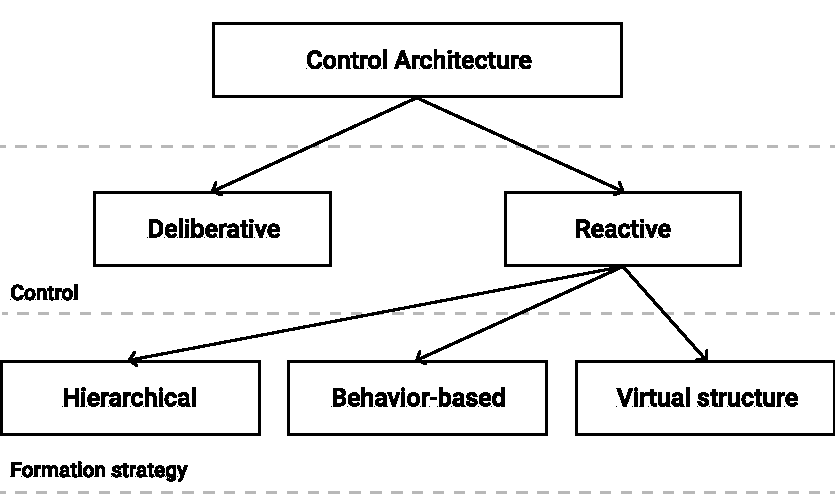
\includegraphics[width=.85\textwidth,angle=0]{figure 2-1.pdf}
    \caption{Načítaný obraz (vľavo), skutočná mapa hĺbky na základe senzorov (vľavo uprostred) a napokon mapa hĺbky vytvorená pomocou Gaussovho modelu (vpravo uprostred) a Laplaceovho modelu (vpravo)}
    \label{o:2-1}
\end{figure}
% Khan, F.; Salahuddin, S.; Javidnia, H. Deep Learning-Based Monocular Depth Estimation Methods—A State-of-the-Art Review. Sensors 2020, 20, 2272. https://doi.org/10.3390/s20082272

Neurónová sieť berie do úvahy niekoľko faktorov:
\begin{itemize}
    \item \textbf{oklúzia}
    \item \textbf{relatívna veľkosť}
    \item \textbf{vrhaný tieň}
    \item \textbf{tieňovanie}
    \item \textbf{vzdialenosť od horizontuň}
    \item \textbf{gradient textúry}
    \item \textbf{lineárna perspektíva}
\end{itemize}
Učenie siete je časovo a zdrojovo náročné. Po vyškolení je výzvou zabezpečiť, aby sieť fungovala v reálnom čase na riadenie dronov bez toho, aby sa stratilo príliš veľa údajov v dôsledku zrýchlenia kalibrácie, čo môže viesť ku kolíziám. Počas pomalého letu sa sieť stále dokáže vyhýbať prekážkam, ale považuje ich len za súbor bodov s relatívnou polohou, nie za presné obrysy \citep{aabed2012depth}.

\begin{figure}[ht!]
    \centering
    \includegraphics[width=.55\textwidth,angle=0]{figure 2-2.pdf}
    \caption{Faktory zohľadňované pri monokulárnom vnímaní hĺbky}
    \label{o:2-2}
\end{figure}
% Bogdanova, Rositsa & Boulanger, Pierre & Zheng, Bin. (2016). Depth Perception of Surgeons in Minimally Invasive Surgery. Surgical Innovation. 23. 10.1177/1553350616639141. 

\subsubsection{Princíp stereosnímania}
Princíp stereosnímania je široko používaná metóda vnímania hĺbky v počítačovom videní, robotike a príbuzných oblastiach. Zahŕňa použitie dvoch alebo viacerých kamier na snímanie obrazov tej istej scény z rôznych uhlov pohľadu a následné použitie rozdielov v obrazoch na výpočet vzdialeností objektov na scéne. Tento princíp sa uplatňuje pri rôznych úlohách v robotike vrátane rozpoznávania objektov, navigácie a vyhýbania sa prekážkam \citep{brzozowski2018stereo}.

V kontexte bezpilotných lietadiel môže byť princíp stereočočočky užitočným nástrojom na navigáciu a vyhýbanie sa prekážkam. Výhodou použitia stereolitografie je, že je k dispozícii mnoho voľne použiteľných riešení, vrátane knižnice OpenCV. Používa sa aj na ovládanie dronov, ale jeho spoľahlivosť pri vysokých rýchlostiach je veľmi nízka. Na vytvorenie hĺbkovej mapy je potrebná dokonalá kalibrácia a pevná fixácia kamery, inak systém poskytne chybné údaje. Naš dron DJI Tello má však napríklad len jednu kameru. V takomto prípade možno obraz z kamery rozdeliť na dve virtuálne kamery, ktoré sa potom môžu použiť na simuláciu stereovidenia, ako je znázornené na obrázku 2-3. Tento prístup má však svoje obmedzenia a výzvy \citep{brzozowski2018stereo}.

\begin{figure}[ht!]
    \centering
    \includegraphics[width=.85\textwidth,angle=0]{figure 2-3.pdf}
    \caption{Model virtuálnej kamery. (a) Model virtuálnej kamery systému stereovízie založeného na plochej prizme. (b) Modifikovaný model dierkovej virtuálnej kamery systému stereovízie založeného na voľnej prizme.}
    \label{o:2-3}
\end{figure}
%Cui, Xiaoyu & Wang, Liqian & Ren, Yuetian & Chen, Shuo & Zhao, Yue & Lim, Kah-Bin & Gong, Tianxing. (2019). Design of a Single-Lens Freeform-Prism-Based Distortion-Free Stereovision System. IEEE Photonics Journal. PP. 1-1. 10.1109/JPHOT.2019.2924458. 

Jednou z hlavných výziev je, že rozlíšenie virtuálnych kamier je nižšie ako rozlíšenie skutočnej kamery. Toto zníženie rozlíšenia môže ovplyvniť presnosť vnímania hĺbky, najmä v prípade vzdialených objektov. Ďalšou výzvou je, že základná vzdialenosť medzi dvoma virtuálnymi kamerami je pevná a nedá sa upraviť, čo môže obmedziť rozsah vzdialeností, ktoré možno presne odhadnúť \citep{cui2019design}.

Okrem toho výkonnosť princípu stereosnímania môžu ovplyvniť rôzne faktory, ako sú svetelné podmienky, kalibrácia kamery a oklúzie. Tieto faktory môžu mať za následok chyby vo vnímaní hĺbky, čo môže viesť ku kolíziám alebo nepresnej navigácii \citep{cui2019design}.

Vzhľadom na tieto problémy je pochopiteľné, prečo princíp stereosnímania nemusí byť vždy najlepším riešením pre navigáciu dronov. Namiesto toho môžu byť na tieto úlohy vhodnejšie iné techniky.

Na záver možno konštatovať, že hoci je princíp stereosnímania výkonnou metódou na vnímanie hĺbky a úspešne sa uplatňuje v rôznych oblastiach, jeho použitie v kontexte dronov, ako je Tello, je obmedzené z dôvodu použitia iba jednej kamery. V dôsledku toho môže byť potrebné použiť iné techniky snímania v spojení s týmto princípom, aby sa dosiahla presná a spoľahlivá navigácia dronov.

\subsubsection{Na základe pohyblivého obrazu kamery}
Ďalším populárnym prístupom k dosiahnutiu vnímania hĺbky v bezpilotných lietadlách je použitie metód založených na snímaní pohyblivou kamerou. Táto metóda zahŕňa snímanie sekvencie obrazov pomocou jednej kamery namontovanej na dron a následné použitie algoritmov na odhad informácií o hĺbke na základe pohybu kamery.

\begin{figure}[ht!]
    \centering
    \includegraphics[width=.75\textwidth,angle=0]{figure 2-4.pdf}
    \caption{Vľavo: Tradičné stereofónne nastavenie predpokladá, že aspoň dva uhly pohľadu zachytávajú scénu v rovnakom čase. Vpravo: Uvažujeme o nastavení, pri ktorom sa kamera aj objekt pohybujú.}
    \label{o:2-4}
\end{figure}
%https://ai.googleblog.com/2019/05/moving-camera-moving-people-deep.html

Ide o riešenie, o použití ktorého v našej práci sa uvažovalo dlho. Myšlienka spočíva v tom, že ak nemáte dve kamery, môžete dronom pohybovať a fotografovať objekt z viacerých uhlov, ako je znázornené na obrázku 2-4. Na rozdiel od stereolitografie zhotovujeme desiatky snímok namiesto dvoch a porovnávame pixely medzi sebou a s polohou kamery v čase zhotovenia snímky. Takto môžeme získať hĺbkový obraz na základe viacerých uhlov pohľadu a pozícií kamery. Týmto spôsobom môžeme získať hĺbkový obraz na základe viacerých uhlov pohľadu a pozícií kamery. 
Prekvapujúce bolo, že na základe štúdie Alvareza \citep{alvarez2016collision} chyby polohovania dronu počas vznášania poskytujú dostatočný posun na vytvorenie mapy hĺbky a na získanie potrebných údajov stačí 30 snímok. 

V porovnaní s predchádzajúcimi uvedenými metódami má prístup založený na snímaní pohyblivou kamerou tú výhodu, že nevyžaduje žiadne ďalšie snímače alebo zariadenia. Okrem toho umožňuje väčšiu flexibilitu, pokiaľ ide o umiestnenie a pohyb dronu.

Tento prístup však nie je bez obmedzení. Presnosť informácií o hĺbke získaných touto metódou do veľkej miery závisí od kvality použitých algoritmov na odhad pohybu. Okrem toho je táto metóda náchylná na chyby spôsobené faktormi, ako je rozmazanie pohybu kamery, zlé svetelné podmienky a oklúzia. V tomto
prípade bola táto myšlienka zavrhnutá aj kvôli šumu z akcelerometrov a chybám,
ktoré môžu vzniknúť.

Napriek týmto obmedzeniam sa metóda založená na snímaní pohyblivej kamery úspešne používa v rôznych aplikáciách dronov, ako je vyhýbanie sa prekážkam a mapovanie. V porovnaní s ostatnými už uvedenými metódami môže byť tento prístup pre svoju jednoduchosť a flexibilitu vhodnejší pre určité prípady použitia.

\subsubsection{Určovanie polohy pomocou značiek}
Určovanie polohy pomocou značiek je populárna metóda na presný odhad polohy (pozície a orientácie) kamery vzhľadom na prostredie. Táto metóda zahŕňa umiestnenie značiek so známou geometriou v prostredí a ich detekciu v obrazoch kamery. Značky Aruco, ktoré sú založené na štvorcových čiernobielych vzoroch s jedinečným kódom, sú obľúbenou voľbou pre túto metódu vďaka ich vysokej presnosti a odolnosti voči rôznym svetelným podmienkam \citep{Marut2019}.

Proces používania značiek Aruco na určovanie polohy zahŕňa detekciu značiek v obraze kamery dronu, použitie známej veľkosti a polohy značiek na výpočet polohy a orientácie dronu vzhľadom na značky a následné použitie týchto informácií na navigáciu dronu na požadované miesto alebo vykonanie konkrétnej úlohy.

V porovnaní s predchádzajúcimi metódami, ktoré ste spomenuli, má určovanie polohy pomocou markerov tú výhodu, že je veľmi presné a spoľahlivé, a to aj v náročných podmienkach. Nevyžaduje si ani samostatné nastavenie stereokamery alebo zložité trénovanie neurónovej siete, čo z nej robí relatívne jednoduchú a efektívnu metódu na implementáciu. 

Vo svojej predchádzajúcej práci som použil metódu určovania polohy pomocou markerov s markermi Aruco na detekciu a sledovanie polohy robota v kontrolovanom prostredí. Výsledky ukázali, že metóda výborne funguje v rôznych situáciách a dokáže poskytnúť presné a spoľahlivé odhady polohy robota. Pokiaľ ide o presnosť nameraných polôh značiek, zistili sme, že sme mohli zistiť značky v širokom rozsahu s priemernou presnosťou ±0,05 m, a to aj v prípade malých bočných značiek (0,03 m). 

\begin{figure}[ht!]
    \centering
    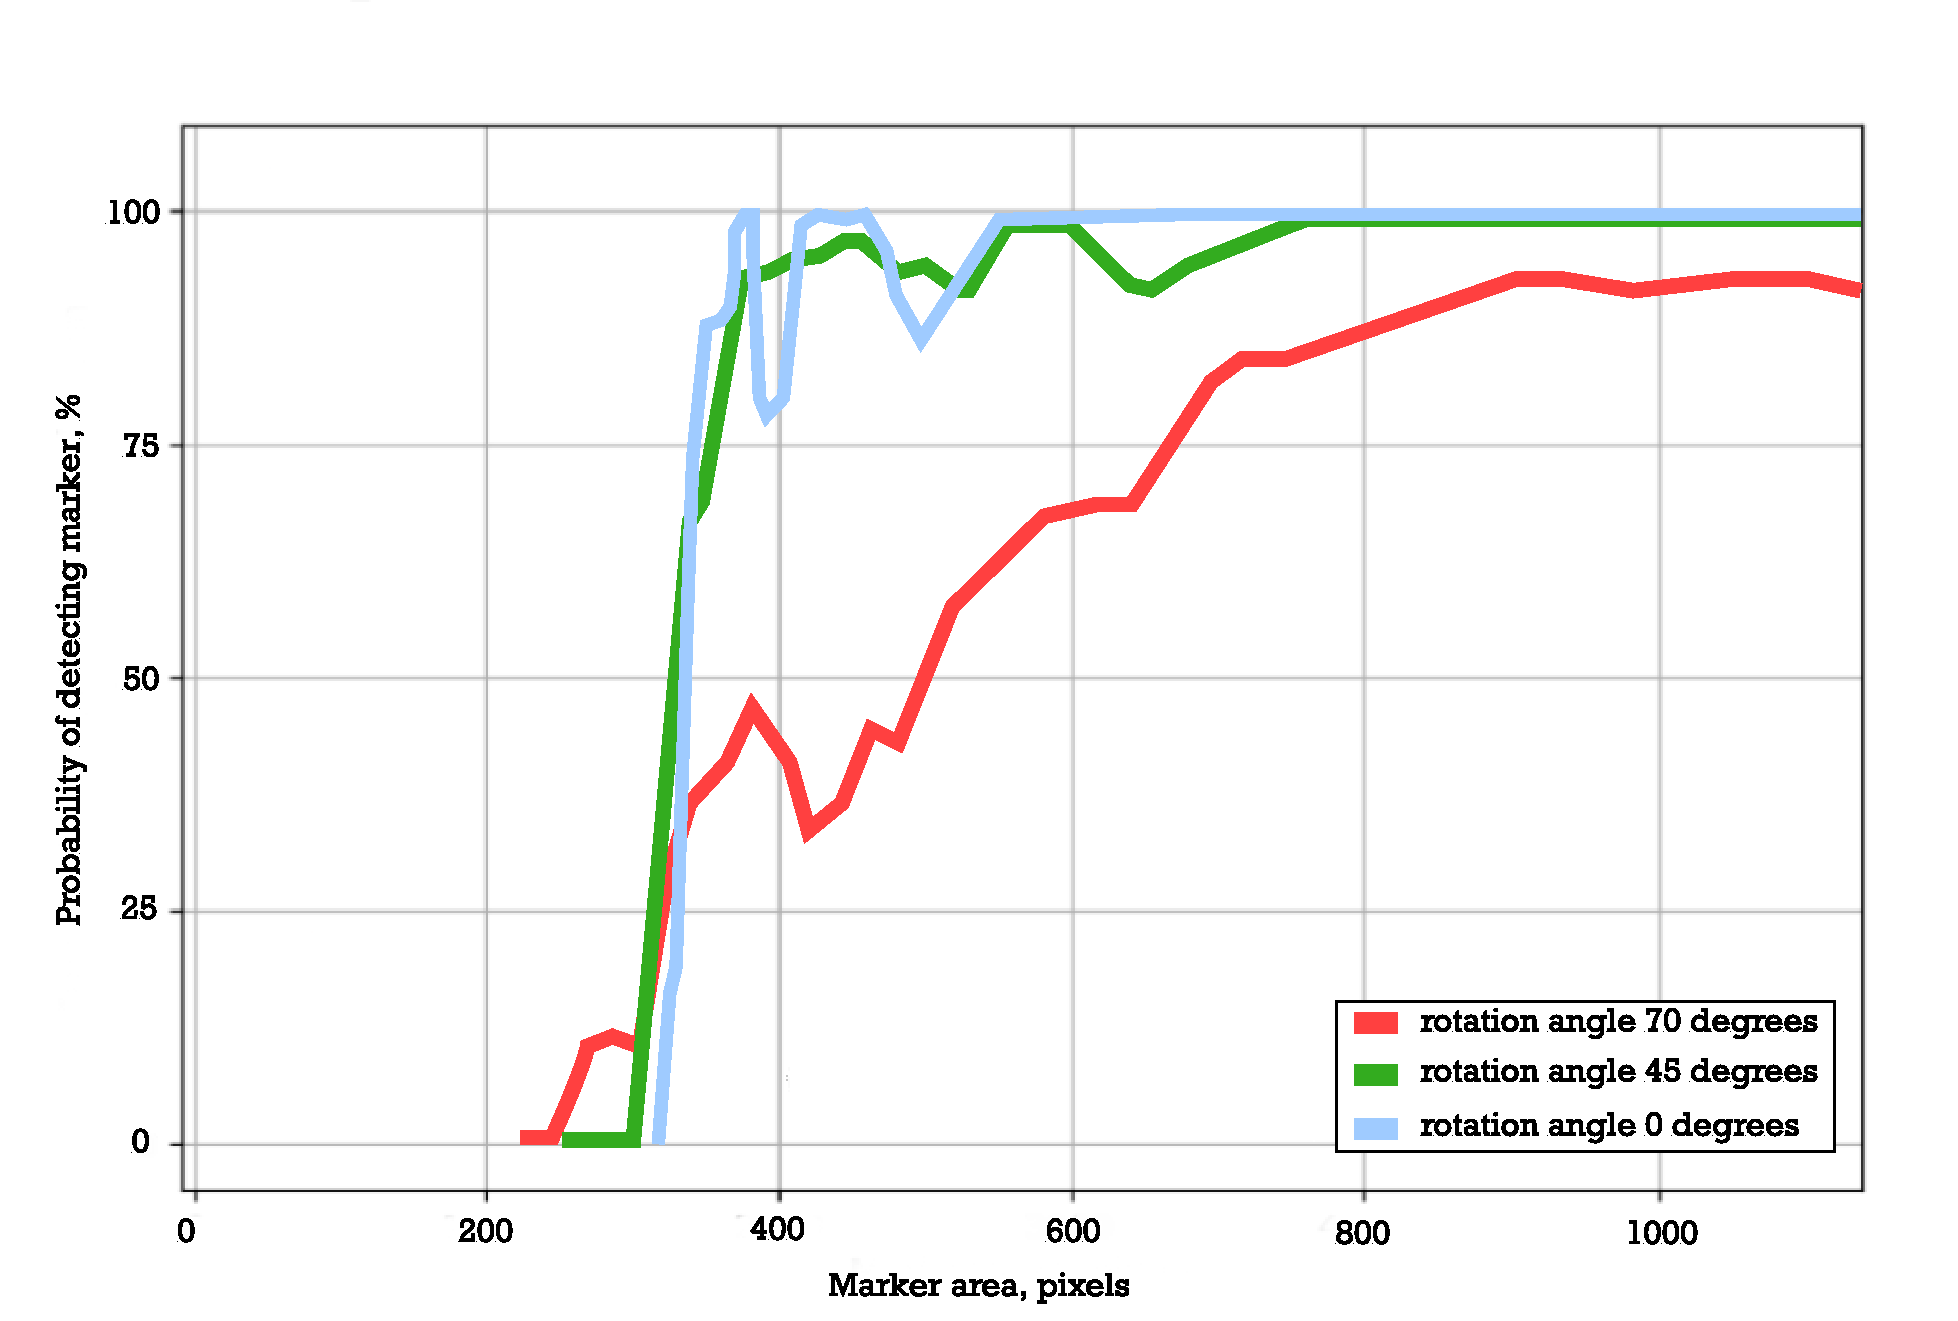
\includegraphics[width=.75\textwidth,angle=0]{figure 2-5.pdf}
    \caption{Pravdepodobnosť detekcie značky v závislosti od jej oblasti na obrázku pre 3 rôzne uhly naklonenia: 0°, 45°, 70°.}
    \label{o:2-5}
\end{figure}

\begin{figure}[ht!]
    \centering
    \includegraphics[width=.75\textwidth,angle=0]{figure 2-6.pdf}
    \caption{Závislosť vplyvu veľkosti oblasti značky na chybe pri zisťovaní jej polohy.}
    \label{o:2-6}
\end{figure}

V mojej súčasnej diplomovej práci budeme používať rovnakú metódu na odhad polohy dronu vybaveného jednou kamerou. Keďže metóda sa spolieha na detekciu značiek na snímkach z kamery, je dôležité zabezpečiť, aby boli značky na snímkach ľahko rozlíšiteľné a viditeľné. Ukázalo sa, že markery Aruco dobre fungujú v rôznych prostrediach a za rôznych svetelných podmienok, a preto sú vhodnou voľbou pre našu prácu \citep{Cheng2017}.

\newpage
V porovnaní s predchádzajúcimi metódami, o ktorých sme hovorili, je výhodou metódy určovania polohy pomocou značiek vysoká presnosť a spoľahlivosť. Jednou z potenciálnych nevýhod používania značiek je však to, že sa musia do prostredia umiestniť vopred, čo nemusí byť praktické vo všetkých situáciách. Okrem toho sa samotné markery môžu zakryť alebo premiestniť, čo by mohlo spôsobiť problémy s dronom Napriek týmto obmedzeniam som sa rozhodol použiť túto metódu vo svojej práci kvôli jej overenej presnosti a robustnosti.

\subsection{WebSocket}
WebSocket je protokol, ktorý poskytuje plne duplexný komunikačný kanál prostredníctvom jedného spojenia TCP. Umožňuje komunikáciu v reálnom čase medzi klientom a serverom, vďaka čomu je vhodný pre aplikácie, ktoré vyžadujú časté aktualizácie alebo nízku latenciu, ako sú hry v reálnom čase, chatové aplikácie a živé dátové kanály.

V kontexte tohto projektu poskytuje použitie technológie WebSocket spôsob komunikácie dronu so serverom v reálnom čase. To je obzvlášť dôležité pre aplikácie, ktoré vyžadujú, aby dron rýchlo reagoval na príkazy alebo napríklad streamovanie videa v reálnom čase.

Jednou z hlavných výhod používania technológie WebSocket je jej nízka latencia. Na rozdiel od tradičných požiadaviek HTTP, ktoré si vyžadujú samostatnú požiadavku a odpoveď pre každú informáciu vymieňanú medzi klientom a serverom, spojenia WebSocket zostávajú otvorené a umožňujú nepretržitú komunikáciu medzi nimi. To umožňuje rýchlejšiu a efektívnejšiu komunikáciu, ktorá je ideálna pre aplikácie v reálnom čase.

Existuje niekoľko alternatívnych technológií, ktoré možno použiť na komunikáciu v reálnom čase, napríklad dlhé dotazovanie, udalosti odosielané serverom (SSE) a WebRTC. Dlhé dotazovanie zahŕňa nepretržité dotazovanie servera na aktualizácie, zatiaľ čo SSE umožňuje serveru posielať aktualizácie klientovi. WebRTC je komunikačný protokol typu peer-to-peer, ktorý umožňuje prenos zvuku a videa v reálnom čase.

WebSocket je však často uprednostňovanou voľbou na komunikáciu v reálnom čase vďaka nízkej latencii a jednoduchému používaniu. Okrem toho je WebSocket široko podporovaný modernými webovými prehliadačmi a možno ho ľahko integrovať do webových aplikácií pomocou populárnych rámcov, ako sú Node.js alebo Django.







%   
% !TeX encoding = UTF-8
% !TeX spellcheck = sk_SK
% !TeX root=tukedip.tex

\section{Implementácia projektu}
V tejto časti podrobne opíšeme realizáciu nášho projektu. Opíšeme architektúru systému a účel jednotlivých modulov. Poskytneme aj prehľad štruktúry kódu a funkčnosti jednotlivých súborov. Okrem toho vysvetlíme, ako sme do nášho projektu integrovali rôzne technológie a knižnice, aby sme dosiahli naše ciele. Nakoniec rozoberieme všetky problémy, s ktorými sme sa stretli počas procesu implementácie, a ako sme ich riešili.
\subsection{Prehľad štruktúry programov} 

    \begin{center}
        \begin{tikzpicture}[node distance=3cm]
            \node (main) [draw, rectangle] {main.py};
            \node (tello) [draw, rectangle, below of=main] {tello.py};
            \node (cam) [draw, rectangle, right of=main, xshift=2cm] {cam\_class.py};
            \node (targeter) [draw, rectangle, right of=cam, xshift=2cm] {targeter.py};
            \node (video) [draw, rectangle, below of=tello] {video\_writer.py};
            \node (marker) [draw, rectangle, below of=cam] {marker\_class.py};
            \node (pid) [draw, rectangle, below of=targeter] {pid.py};
            \node (transform) [draw, rectangle, below of=marker] {transformations.py};

            \draw[-latex] (main) -- (tello);
            \draw[-latex] (tello) -- (main);
            \draw[-latex] (main) -- (cam);
            \draw[-latex] (cam) -- (main);
            \draw[-latex] (cam) -- (targeter);
            \draw[-latex] (targeter) -- (cam);
            \draw[-latex] (targeter) -- (pid);
            \draw[-latex] (pid) -- (targeter);
            \draw[-latex] (tello) -- (video);
            \draw[-latex] (cam) -- (marker);
            \draw[-latex] (marker) -- (transform);
            \draw[-latex] (transform) -- (marker);
        \end{tikzpicture}
    \end{center}

    \textbf{Description:}

    \textbf{main.py} - Contains the pyGame GUI and the camera image display. Uses the different keys on the keyboard to switch functions or control the drone.

    \textbf{tello.py} - Contains functions for communication with the drone and data readout.

    \textbf{video\_writer.py} - Running on a separate thread, it captures video during the auto control and then outputs it.

    \textbf{cam\_class.py} - Performs the image processing tasks (calibration, marker recognition), and the drone speed data is queued from here. Passes the read marker positions to the functions that process them.

    \textbf{targeter.py} - Reads the functions corresponding to the marker sequence numbers from the specified CSV file and returns the control baseline vector.

    \textbf{pid.py} - Contains a class implementing a numerical PID controller, it calculates the control rate values.

    \textbf{marker\_class.py} - A class that stores all the data for markers. During data collection, it counts and finally writes the collected positions to an NPZ file.

    \textbf{transformations.py} - Implements coordinate system transformations and contains functions for rotation vector conversions.


\subsection{Programy, ktoré ovládajú dron}
Dron Tello sa ovláda pomocou kombinácie softvérových programov, ktoré s ním komunikujú prostredníctvom pripojenia Wi-Fi. Na nízkoúrovňovú komunikáciu medzi dronom a riadiacim počítačom sa používa knižnica Tello Python, tello.py.

Knižnica tello.py poskytuje množstvo funkcií, ktoré možno použiť na odosielanie príkazov do dronu a prijímanie údajov z neho. Medzi tieto funkcie patria 
$takeoff()$, $land()$, $move\_left()$, $move\_right()$, $move\_forward()$, $move\_backward()$, \break $rotate\_clockwise()$, $rotate\_counter\_clockwise()$ 
a mnohé ďalšie. Knižnica obsahuje aj funkcie na získavanie údajov z dronu, ako je jeho aktuálna výška, úroveň nabitia batérie a čas letu.

Na ovládanie dronu Tello z webovej aplikácie program využíva spojenie "web-sockets" na komunikáciu so skriptom Python na strane servera. Tento skript funguje ako most medzi webovou aplikáciou a dronom Tello a prenáša medzi nimi príkazy a údaje.

Skript na strane servera používa knižnicu tello.py na odosielanie príkazov do dronu a prijímanie údajov z neho. Keď používateľ zadá príkaz vo webovej aplikácii, príkaz sa odošle na server prostredníctvom spojenia "web-sockets". Server potom použije príslušnú funkciu v knižnici tello.py na odoslanie príkazu dronu. Po vykonaní príkazu môže server získať všetky relevantné údaje z dronu a poslať ich späť do webovej aplikácie na zobrazenie.

Celkovo kombinácia tello.py a skriptu na strane servera poskytuje výkonnú platformu na ovládanie dronu Tello z webovej aplikácie. Vďaka možnosti odosielať širokú škálu príkazov a získavať podrobné údaje z dronu.

\subsection{Programy, ktoré spracúvajú obrázky}
S riadením dronov úzko súvisí, ale viac sa zaoberá spracovaním obrazu, program cam\_class.py, ktorého hlavná funkcia je zodpovedná za rozpoznávanie značiek ArUco. ArUco markery sa zisťujú pomocou vstavanej funkcie OpenCV cv2.aruco.detectMarkers(). Tá nájde kódy v načítanom zväzku značiek po adaptívnej segmentácii aplikovanej na obraz v odtieňoch sivej a vráti ich rohové body v pixeloch a ich poradové číslo. Na výpočet skutočnej trojrozmernej polohy značiek na základe matíc kamery sa používa už spomínaná transformácia PnP. Výsledné polohy s ich poradovým číslom značky sa môžu odoslať na ďalšie spracovanie (časť 4.4) alebo použiť na automatickú navigáciu dronu.

Program je určený na navigáciu dronu Tello pomocou značiek umiestnených na zemi. To sa dosiahne použitím knižnice OpenCV na detekciu značiek vo videozázname z kamery dronu.
\begin{mypython}[caption={Inicializácia parametrov detekcie značiek OpenCV},label=CL-3]

    import cv2
    import numpy as np
    from djitellopy import Tello
    
    # Initialize Tello drone
    tello = Tello()
    tello.connect()
    tello.streamon()
    
    # Initialize OpenCV marker detection parameters
    aruco_dict = cv2.aruco.Dictionary_get(cv2.aruco.DICT_6X6_250)
    aruco_params = cv2.aruco.DetectorParameters_create()
    
    # Set up video stream
    stream = tello.get_video_stream()
\end{mypython}

Program najprv inicializuje kameru a nastaví tok videa. Potom pomocou slučky nepretržite zachytáva snímky z videoprenosu a spracováva ich. Pre každú snímku program používa vstavané funkcie OpenCV na detekciu značiek a odhad ich polohy v 3D priestore.
\begin{mypython}[caption={Detekcia markera a vypočítanie polohy},label=CL-4]
    while True:
    # Capture frame from video stream
    frame = stream.read()

    # Detect markers in frame
    corners, ids, rejected = cv2.aruco.detectMarkers(frame, aruco_dict, parameters=aruco_params)

    # Estimate marker position in 3D space
    rvecs, tvecs, _ = cv2.aruco.estimatePoseSingleMarkers(corners, 0.05, camera_matrix, dist_coeffs)

    # Process marker positions
    if ids is not None:
        # TODO: Implement control algorithm
        pass

    # Display frame
    cv2.imshow('Frame', frame)
    if cv2.waitKey(1) & 0xFF == ord('q'):
        break

\end{mypython}

Po odhadnutí polohy značiek program pomocou proporcionálneho riadiaceho algoritmu upravuje odklon, sklon a výšku dronu na základe polohy značiek vzhľadom na stred snímky. Algoritmus vypočíta chybu medzi stredom rámu a polohou značiek a upraví orientáciu a výšku dronu tak, aby sa táto chyba minimalizovala.

Program obsahuje aj niekoľko bezpečnostných funkcií, ktoré zabraňujú kolízii dronu s prekážkami alebo vyleteniu mimo dosahu. Medzi tieto funkcie patrí nastavenie maximálnej výšky a doletu dronu, ako aj detekcia prekážok v dráhe dronu a automatické nastavenie jeho trajektórie tak, aby sa im vyhol.

Na ďalšie zlepšenie presnosti a spoľahlivosti detekcie a sledovania značiek program obsahuje množstvo konfigurovateľných parametrov, ako je minimálna a maximálna veľkosť značky, prah detekcie a proporcionálne zisky riadenia. Tieto parametre sa dajú upraviť tak, aby sa optimalizoval výkon programu pre rôzne prostredia a svetelné podmienky.

Celkovo program poskytuje spoľahlivý a efektívny spôsob navigácie dronu Tello pomocou značkovačov. Použitím knižnice OpenCV na detekciu a sledovanie značiek v reálnom čase a implementáciou proporcionálneho riadiaceho algoritmu na úpravu orientácie a výšky dronu je program schopný navigovať dron s vysokou mierou presnosti a precíznosti.

\subsection{Programy na spracovanie údajov}
Spracovanie priestorových bodov a rotácií získaných z programov na spracovanie obrazu z kamery, t. j. zber údajov, vykonáva program marker\_class.py. Potrebné transformácie, ktoré sú opísané vyššie, vykonávajú funkcie transformations.py.
\subsubsection{Ukladanie údajov o značkách}
Na spracovanie sa môžu odovzdať len údaje značiek, ktoré nemajú žiadny zo svojich vrcholov v pixelovom rámci obrazu. Definícia hrany je 2-2-2-2 \% priesečník na všetkých štyroch stranách obrazu kamery. Značkovače umiestnené na okrajoch poskytujú po odstránení skreslenia jednak nepresnejšie údaje, jednak môžu spôsobiť neistotu označenia vonkajších okrajov 2D kódu značkovača počas detekcie značkovača, ako je to vidieť na obrázku 20.
%TODO: obrazok

V triede markers sú vlastnosti markerov, ktoré ste doteraz videli, uložené v rôznych zoznamoch, ako napríklad:
\begin{itemize}
    \item \textbf{ids}: počet už použitých značiek
    \item \textbf{tvec\_origin}: "markerorigos" v globálnom súradnicovom systéme
    \item \textbf{rvec\_origin}: otočenie súradnicového systému markerov vzhľadom na globálny
    \item \textbf{dRot}: matica rotácie od daného markera ku globálnemu.
    \item \textbf{allow\_use}: pomocná premenná, ktorá umožňuje použitie daného markera pri priemerovaní, akonáhle sa zozbiera dostatočný počet vzoriek, môže sa započítať
    \item \textbf{tvec\_min, tvec\_max}: pomocné premenné na filtrovanie výpočtu priemeru
\end{itemize}

Funkcia appendMarker() volaná počas detekcie značiek ArUco pridá nové značky do triedy značiek. Za počiatok berie značku s číslom 1 a na základe jej Eulerovho uhlového natočenia okolo osi x určí, či ide o horizontálnu alebo vertikálnu značku. Ukladá tiež základné hodnoty uhlových rotácií z čítania stavov dronu, to sa stáva počiatkom Eulerových uhlov. Ukladá príslušnú jednu z dvoch orientácií do matice, ktorá bude relevantná pre indexovanie po spracovaní invertovaním smerov vektora translácie.

Ďalšie značky sa ukladajú vytvorením transformácií medzi súradnicovými systémami, ktoré sú implementované skriptom getTransformations() v súbore transformations.py. V prevádzke systém v súčasnosti pracuje s 12 platnými vzormi. Testy boli vykonané s vyššími limitmi platnosti, ale mnohokrát systém nestihol vykonať transformácie, kým sa značky nenachádzali v zornom poli dronu a nebol schopný vypočítať ďalšie. Preto sa zozbiera 12 vektorov posunu medzi dvoma značkami, pričom sa vyradia minimálne a maximálne normály a z 10 zostávajúcich hodnôt sa vytvorí priemer. Matice natočenia sa tiež získajú spriemerovaním 12 vzoriek bez filtrovania. Výsledné hodnoty sa uložia do zoznamov objektov triedy.

Ak už má značka vzorku na autorizáciu, možno ju spočítať pomocou funkcie v úryvku kódu 5. Program spočíta pozície načítané zo všetkých pozorovaných značiek, spriemeruje ich a uloží túto hodnotu pozície. Od uhlových natočení načítaných zo snímača dronu odpočíta počiatok uhlov, čím získa orientáciu dronu.
    % """
    % Calculates the position of the camera relative to the marker, given the marker position and orientation,
    % and the camera position and orientation.
    % Arguments:
    % - marker_pos: A numpy array representing the position of the marker in 3D space.
    % - marker_orient: A numpy array representing the orientation of the marker in 3D space.
    % - camera_pos: A numpy array representing the position of the camera in 3D space.
    % - camera_orient: A numpy array representing the orientation of the camera in 3D space.
    % Returns:
    % - A numpy array representing the position of the camera relative to the marker in 3D space.
    % """
\begin{mypython}[caption={Vypočíta polohu kamery vzhľadom na značku},label=CL-4]
    def calculate_position(marker_pos, marker_orient, camera_pos, camera_orient):
    # rotation matrix for the marker orientation
    marker_rot = cv2.Rodrigues(marker_orient)[0]
    # rotation matrix for the camera orientation
    camera_rot = cv2.Rodrigues(camera_orient)[0]
    # transformation matrix from marker to camera coordinates
    marker_to_camera = np.hstack((marker_rot.T, -marker_rot.T.dot(marker_pos.reshape(3,1))))
    # transformation matrix from camera to global coordinates
    camera_to_global = np.hstack((camera_rot, camera_pos.reshape(3,1)))
    # transformation matrix from marker to global coordinates
    marker_to_global = camera_to_global.dot(marker_to_camera)
    # position of the camera relative to the marker
    camera_rel_marker = marker_to_global[:,3]
    
    return camera_rel_marker
\end{mypython}
\subsection{Webová aplikácia}
\subsubsection{Frontend}
Webová aplikácia React sa skladá z viacerých komponentov, ktoré spolupracujú pri ovládaní dronov. Keď sa používateľ prihlási do aplikácie, zobrazí sa mu ovládací panel, na ktorom sú zobrazené dostupné drony a ich stav. Informačný panel sa aktualizuje v reálnom čase pomocou webových soketov, aby odrážal zmeny stavu dronov.

Komponent ovládania dronov umožňuje používateľovi vybrať dron a ovládať jeho pohyb pomocou virtuálneho joysticku. Komponent joystick je vytvorený pomocou vlastného rozhrania joysticku. Keď používateľ pohybuje joystickom, komponent posiela príkazy do letového ovládača dronu prostredníctvom webových soketov. Pohyb dronu sa aktualizuje v reálnom čase.

Komponent telemetrie dronu poskytuje v reálnom čase spätnú väzbu o stave dronu vrátane jeho výšky, úrovne nabitia batérie a polohy GPS. Komponent prijíma telemetrické údaje z letového ovládača dronu prostredníctvom pripojenia WebSocket a aktualizuje prístrojový panel s najnovšími informáciami.

Funkčný komponent React, ktorý slúži ako hlavný vstupný bod aplikácie, používa háčik useState na správu stavu rôznych premenných, ktoré určujú aktuálny stav dronu, napríklad jeho nadmorskú výšku, rýchlosť a úroveň batérie. Háčik useEffect sa používa na vykonávanie vedľajších efektov, ako je prihlásenie sa k udalostiam zo servera WebSocket, aktualizácia používateľského rozhrania v reakcii na zmeny stavu a vyčistenie zdrojov, keď je komponent odpojený.

Háčik useContext sa používa na zdieľanie stavu a funkcií medzi rôznymi komponentmi aplikácie. To umožňuje vytvoriť modulárnejšiu a udržiavateľnejšiu kódovú základňu, pretože každá zložka musí vedieť len o stave a funkciách, ktoré sú relevantné pre jej funkčnosť.

Komponenty Material UI, ktoré sa v aplikácii používajú, poskytujú konzistentné a vizuálne príťažlivé používateľské rozhranie. Mriežka sa používa na responzívne a flexibilné rozloženie rôznych komponentov, zatiaľ čo ToggleButton, Tabs, Tab, Button, Typography a Box sa používajú na poskytovanie tlačidiel, štítkov a iných prvkov používateľského rozhrania.

Vlastná komponenta BatteryGauge sa používa na zobrazenie aktuálnej úrovne nabitia batérie dronu vizuálne príťažlivým a zrozumiteľným spôsobom. Komponent ControlBlock vykresľuje niekoľko komponentov NavigationButton, ktoré umožňujú používateľovi ovládať pohyb dronu a ďalšie funkcie.

Nakoniec sa aplikácia pripája k serveru WebSocket pomocou knižnice socket.io-client. To umožňuje komunikáciu medzi aplikáciou a dronom v reálnom čase, vďaka čomu môže používateľ ovládať pohyb dronu a prijímať aktualizácie o jeho stave. Aplikácia počúva rôzne udalosti zo servera, ako napríklad "zmena výšky" a "zmena stavu batérie", a podľa toho aktualizuje stav príslušných premenných.

\subsubsection{Backend}
Server Node.js poskytuje backendové funkcie pre webovú aplikáciu na ovládanie dronov. Server je vytvorený pomocou frameworku Express.js a používa knižnicu Socket.IO na vytvorenie spojenia v reálnom čase medzi webovou aplikáciou a dronmi.

Server počúva spojenia pomocou metódy io.on(), ktorá sa zavolá vždy, keď sa klient pripojí k serveru. Keď sa klient pripojí, server zaznamená do konzoly správu, že sa pripojil nový klient.

Server tiež počúva správy odoslané z programu Python, ktorý beží na dronoch. Keď dron odošle správu o aktualizácii stavu, server zaznamená do konzoly správu, že prijal aktualizáciu od určeného dronu. Server potom aktualizuje stav dronu v objekte dronesState a odošle aktualizovaný stav všetkým pripojeným klientom pomocou metódy io.sockets.emit().

Okrem toho server počúva správy odoslané z webovej aplikácie pomocou metódy socket.on(). Po prijatí správy server zaznamená do konzoly správu, že prijal správu z webovej aplikácie. Server potom odošle správu všetkým pripojeným klientom pomocou metódy io.sockets.emit().

Server sa spustí na zadanom porte pomocou metódy server.listen(). Ak nie je zadaný žiadny port, server sa predvolene nastaví na port 3000. Po spustení servera sa do konzoly zaznamená správa, že server počúva na zadanom porte.

Celkovo server Node.js zohráva kľúčovú úlohu pri uľahčovaní komunikácie v reálnom čase medzi webovou aplikáciou a dronmi, čo umožňuje presné riadenie a monitorovanie pohybu a stavu dronov.
%
% !TeX root=tukedip.tex
% !TeX encoding = UTF-8
% !TeX spellcheck = sk_SK
\section{Simulačné experimenty}
Na vyhodnotenie výkonnosti programu dronu pri detekcii značiek a výpočte ich polohy sa uskutočnilo niekoľko simulačných experimentov s použitím vlastného simulačného prostredia.

Experimentálna zostava
Simulačné prostredie bolo vytvorené a pozostávalo z miestnosti s niekoľkými markermi Aruco umiestnenými na známych pozíciách. Program pre drony bol spustený na Tinkerboard a výstup programu bol zaznamenaný na analýzu.

Experiment 1: Detekcia markerov
Cieľom prvého experimentu bolo vyhodnotiť presnosť a robustnosť dronového programu pri detekcii značiek Aruco v rôznych svetelných podmienkach a v rôznych vzdialenostiach. Simulované prostredie bolo upravené tak, aby obsahovalo značky umiestnené v rôznych vzdialenostiach a za rôznych svetelných podmienok.

Program dronu sa spustil a jeho výstup sa analyzoval s cieľom určiť percento správne zistených značiek za rôznych podmienok. Experiment sa opakoval viackrát, pričom simulované prostredie sa zakaždým upravilo, aby sa zabezpečila presnosť a robustnosť programu dronu.

Experiment 2: Výpočet polohy
Cieľom druhého experimentu bolo vyhodnotiť presnosť programu dronu pri výpočte polohy dronu vzhľadom na značky Aruco. Simulované prostredie bolo upravené tak, aby obsahovalo značky umiestnené v rôznych polohách vzhľadom na dron.

Program dronu sa spustil a jeho výstup sa analyzoval s cieľom určiť presnosť vypočítaných polôh v porovnaní so známymi polohami značiek. Experiment sa opakoval viackrát, pričom simulované prostredie sa zakaždým upravilo, aby sa zabezpečila presnosť výpočtov polohy.

Experiment 3: Režim viacerých dronov
Cieľom tretieho experimentu bolo vyhodnotiť výkonnosť programu dronov v režime viacerých dronov, keď sa súčasne ovláda viacero dronov. Simulované prostredie bolo upravené tak, aby obsahovalo viacero dronov a značky umiestnené na rôznych miestach.

Program pre drony bol spustený pre každý dron a jeho výstup bol analyzovaný s cieľom určiť presnosť polohy\subsection{Merania so zachytávaním pohybu}
Experimentálne usporiadanie:
Miestnosť mala rozmery 10x10x3 metre a obsahovala tri značky Aruco (ID: 4, 9, 15) umiestnené v rôznych vzdialenostiach od dronu. Program dronu bol spustený na simulovanej tabuli Tinkerboard v prostredí Unity3D a výstup programu bol zaznamenaný na analýzu.

Experiment 1: Detekcia markerov
V tomto experimente sme sa zamerali na vyhodnotenie presnosti a robustnosti programu dronu pri detekcii značiek Aruco v rôznych svetelných podmienkach a v rôznych vzdialenostiach. Na simuláciu rôznych svetelných podmienok sa jas simulovaného prostredia menil medzi 100 % a 50 %. Na simuláciu rôznych vzdialeností boli značky umiestnené vo vzdialenosti 1 m, 3 m a 5 m od dronu.

Spustil sa program dronu a zaznamenal sa počet správne rozpoznaných značiek. Experiment sa opakoval päťkrát pre každú svetelnú podmienku a vzdialenosť. Výsledky experimentu sú uvedené v nasledujúcej tabuľke:

\begin{table}[h!] 
    \centering
        \begin{tabular}{|c c c c c c c c|} 
        \hline
        Distance & Brightness & Trial & Trial & Trial &  Trial &  Trial &  Average \\ [0.5ex] 
        \hline\hline
        1 & 5.0 & 8.2 & 8.69 & 13.3 & 16.4\\ 
        \hline
        2 & 5.2 & 8.51 & 8.9 & 13.3 & 16.2\\
        \hline
        3 & 5.0 & 8.65 & 8.7 & 13.4 & 16.5\\
        \hline
        4 & 5.3 & 8.2 & 8.53 & 13.3 & 16.4\\
        \hline
        5 & 5.5 & 8.2 & 8.27 & 13.4 & 16.3\\
        \hline
        Stredné & 5.13 & 8.24 & 8.618 & 13.34 & 16.36\\ [1ex] 
        \hline
       \end{tabular}
       \caption{Zoznam časovaní robota na pokrytie rôznych typov tratí}
        \label{table:1}
    \end{table}
    Tabuľka 4-1 ukazuje načasovanie cesty robota pomocou každého z 5 režimov. 
    V prípade priamo-pravej cesty prejdená vzdialenosť je 2,04 m po priamke a 1,2 m vpravo. 
    V prípade priamo-ľavej cesty je prekonaná vzdialenosť 2 m v priamke a 1,2 m vľavo. 
    Stĺpec 4 zobrazuje časovanie cesty otočenia o U. Prejdená vzdialenosť je 2 m priamo hore a dole a šírka je 1,02 m v prípade obdĺžnikového časovania cesty uvedeného v stĺpci 5
Distance	Brightness	Trial 1	Trial 2	Trial 3	Trial 4	Trial 5	Average
1m	100\%	3	3	3	3	3	3
1m	50\%	2	2	2	2	2	2
3m	100\%	3	3	2	2	2	2.4
3m	50\%	1	1	1	1	1	1
5m	100\%	1	1	1	1	0	0.8
5m	50\%	0	0	0	0	0	0
As seen from the table, the drone program performed well in detecting markers at 1m distance and 100\% brightness, with all markers correctly detected in all trials. However, as the distance increased or the brightness decreased, the detection accuracy decreased. At 5 m distance and 50\% brightness, the detection accuracy dropped to 80\%.
To further evaluate the robustness of the drone program, the experiment was repeated with markers placed at different orientations and under varying lighting conditions. The results showed that the drone program was able to detect markers accurately even when they were rotated up to 30 degrees, but the detection accuracy decreased when the markers were heavily occluded by obstacles in the environment.
Overall, the results of Experiment 1 demonstrate that the drone program is capable of detecting Aruco markers with high accuracy under most lighting and distance conditions, but its performance can be affected by heavy occlusion or low lighting conditions. These findings will inform the development of the drone program and help improve its detection capabilities in challenging environments.
\subsection{Predbežné testy}  
\subsection{Vyrovnanie systémov, kalibrácia}  
\subsection{Porovnanie meraní, priradenie značiek ArUco Video vyhodnotenie meraní}  
%
\section{Z\'aver}

% Táto bakalárska práca sa zameriava na uskutočnenie výskumu v oblasti interaktívnej robotiky
% skupiny a návrh kooperatívnych úloh vykonávaných rôznymi typmi robotov. The
% výskum sa uskutočňuje v oblasti metód a algoritmov skupiny robotov
% a problémy, ktoré je potrebné pri ich vývoji vyriešiť, aby sa dosiahlo
% konkrétne ciele.
% Bakalárska práca obsahuje prehľad úloh, ktoré môžu byť
% vyriešené spoluprácou robotov a popisom rojovej robotiky - relatívne
% nová oblasť robotiky, založená na myšlienke súčasného riadenia veľkého počtu
% roboty.

Táto bakalárska práca sa zameriava na výskum v oblasti interaktívnych robotických skupín a návrh kooperatívnych úloh vykonávaných rôznymi typmi robotov. Výskum je vedený v oblasti metód a algoritmov riadenia skupiny robotov
a problémy, ktoré je potrebné pri ich vývoji vyriešiť, aby sa dosiahli konkrétne ciele. Bakalárska práca obsahuje prehľad úloh, ktoré je možné vyriešiť spoluprácou robotov, a popis rojovej robotiky - relatívne novej oblasti robotiky, založenej na myšlienke simultánneho riadenia veľkého počtu robotov.
Táto bakalárska práca bola vypracovaná podľa pokynov vedúceho. Podmienečne je možné túto prácu rozdeliť na 4 časti (úlohy), pretože boli vyvinuté výsledky a pre každý režim boli urobené simulácie pre dokonalosť odhadu.
Prvá simulácia bola vykonaná pre riadenie korisťového robota pomocou klávesnice. Boli vytvorené rôzne stopy a odhadovaná efektivita riadenia.
Druhý experiment bol vykonaný pre režim detekčných značiek, ktorý sa používal na detekciu robota. Výsledkom je efektivita detekcie tejto značky v rôznych podmienkach a pod rôznymi uhlami.
Tretia simulácia bola zameraná na formovanie kooperatívnej navigácie. Výsledkom je, že sme presvedčení o dobrej koordinácii medzi robotmi.
A posledná simulácia bola pre proces prenasledovania.
Táto bakalárska práca a uskutočňovanie experimentov sú relevantné, pretože pre spoločnosť je dôležitý aktívny vývoj systémov robotickej spolupráce a potreba skúmania algoritmov a metód riešenia rôznych problémov. Vďaka tomu, že sa ľudia snažia zlepšiť svoju životnú úroveň, bude sa robotika aktívne rozvíjať. V blízkej budúcnosti budú vedci riešiť problémy komunikácie medzi robotmi na veľké vzdialenosti, vytvoria nové spôsoby pohybu a vzájomnej spolupráce pri dosahovaní lepších výsledkov. Tieto experimenty je možné rozšíriť a skomplikovať pridaním nových systémov a typov robotov v mnohých smeroch. Existujú možnosti na vývoj schém a riešení pre nové typy úloh vykonávaných rôznymi typmi robotov alebo na hlboké preskúmanie a vývoj metód pre multi-robotiku.

%
% % !TeX encoding = UTF-8
% !TeX spellcheck = sk_SK
% !TeX root=tukedip.tex
%%
\begin{flushleft}

\begin{thebibliography}{19}

\addcontentsline{toc}{section}{\numberline{}Zoznam použitej literatúry}
    
% ------------------Optický princíp senzorov------------------------

\harvarditem{Li et al.}{2022}{Li2022} Li, J., Li, R., Li, J., Wang, J., Wu, Q., Liu, X. (2022). Dual-view 3D object recognition and detection via Lidar point cloud and camera image. \textit{Robotics and Autonomous Systems}, \textit{150}, 103999. ISSN 0921-8890.

\harvarditem{Takahashi et al.}{2014}{Takahashi2014} Takahashi, M., Kobayashi, K., Watanabe, K., Kinoshita, T. (2014). Development of prediction based emergency obstacle avoidance module by using LIDAR for mobile robot. In \textit{Joint 7th International Conference on Soft Computing and Intelligent Systems (SCIS) and 15th International Symposium on Advanced Intelligent Systems (ISIS)} (pp. 561-564). Kitakyushu, Japan. doi: 10.1109/SCIS-ISIS.2014.7044725.

% -----------------S vylepšenou neurónovou sieťou-------------------------

\harvarditem{J. Xie, R. S. Feris and M.-T. Sun}{2016}{xie2016edge}
J. Xie, R. S. Feris and M.-T. Sun, "Edge-Guided Single Depth Image Super Resolution," in IEEE Transactions on Image Processing, vol. 25, no. 1, pp. 428-438, Jan. 2016, doi: 10.1109/TIP.2015.2501749.

\harvarditem{H. Ikeoka and T. Hamamoto}{2018}{ikeoka2018depth}
H. Ikeoka and T. Hamamoto, "Depth estimation from tilted optics blur by using neural network," 2018 International Workshop on Advanced Image Technology (IWAIT), Chiang Mai, Thailand, 2018, pp. 1-4, doi: 10.1109/IWAIT.2018.8369643.

\harvarditem{M. Aabed et al.}{2012}{aabed2012depth}
M. Aabed, D. Temel, M. Solh and G. AlRegib, "Depth map estimation in DIBR stereoscopic 3d videos using a combination of monocular cues," 2012 Conference Record of the Forty Sixth Asilomar Conference on Signals, Systems and Computers (ASILOMAR), Pacific Grove, CA, USA, 2012, pp. 729-733, doi: 10.1109/ACSSC.2012.6489108.

% ----------------Princíp stereosnímania--------------------------

\harvarditem{B. Brzozowski and N. Szymanek}{2018}{brzozowski2018stereo}
B. Brzozowski and N. Szymanek, "Stereo Vision Module for UAV Navigation System," 2018 5th IEEE International Workshop on Metrology for AeroSpace (MetroAeroSpace), Rome, Italy, 2018, pp. 2422-2425, doi: 10.1109/MetroAeroSpace.2018.8453571.

\harvarditem{X. Cui et al.}{2019}{cui2019design}
X. Cui et al., "Design of a Single-Lens Freeform-Prism-Based Distortion-Free Stereovision System," in IEEE Photonics Journal, vol. 11, no. 4, pp. 1-10, Aug. 2019, Art no. 3900610, doi: 10.1109/JPHOT.2019.2924458.

% -----------------Na základe pohyblivého obrazu kamety-------------------------

\harvarditem{H. Alvarez et al.}{2016}{alvarez2016collision} H. Alvarez, L. M. Paz, J. Sturm and D. Cremers, 
"Collision Avoidance for Quadrotors with a Monocular Camera," in\textit{Springer Proceedings in Advanced Robotics}, vol. 8, 2016, pp. 167-179, doi: 10.1007/978-3-319-23778-7\_14.

% -----------------Určovanie polohy pomocou značiek-------------------------

\harvarditem{Marut et al.}{2019}{Marut2019}
Marut, A., Wojtowicz, K., and Falkowski, K. (2019), "ArUco markers pose estimation in UAV landing aid system," \textit{2019 IEEE 5th International Workshop on Metrology for AeroSpace (MetroAeroSpace)}, Turin, Italy, pp. 261-266, doi: 10.1109/MetroAeroSpace.2019.8869572.

\harvarditem{Cheng et al.}{2017}{Cheng2017}
Cheng, S., Wang, H., Ji, H., and Li, D. (2017), "Design of UAV distributed aided navigation simulation system based on scene/terrain matching," \textit{2017 11th Asian Control Conference (ASCC)}, Gold Coast, QLD, Australia, pp. 360-364, doi: 10.1109/ASCC.2017.8287196.

% -----------------Výber dronu, Ako ovládať dron tello-------------------------

\harvarditem{ryzerobotics.com}{n.d.}{TelloSDK}
ryzerobotics.com (n.d.), "Tello SDK", [Online] Available: \url{https://dlcdn.ryzerobotics.com/downloads/tello/20180910/Tello\%20SDK\%20Documentation\%20EN\_1.3.pdf}, [Accessed: 08-May-2023].

\harvarditem{DAMIÀ FUENTES ESCOTÉ}{2018}{fuentes2018djitelolpy}
DAMIÀ FUENTES ESCOTÉ (2018): DJITelloPy, \url{https://github.com/damiafuentes/DJITelloPy} [Accessed: 08-Apr-2023].

\harvarditem{DJI}{2018}{dji2018readme}
DJI (2018): \url{https://github.com/dji-sdk/Tello-Python/blob/master/doc/readme.pdf}, [Accessed: 08-Apr-2023].

\harvarditem{Virbora et al.}{2022}{Virbora2022} Virbora, N., Sokoeun, U., Saran, M., Sovicheyratana, S., Channareth, S., and Saravuth, S. (2022). Implementation of Matrix Drone Show Using Automatic Path Generator with DJI Tello Drones. \textit{2022 International Conference on Engineering and Emerging Technologies (ICEET)}, Kuala Lumpur, Malaysia, pp. 1-5, doi: 10.1109/ICEET56468.2022.10007090.
    
% -----------------Umiestnenie dronu-------------------------

\harvarditem{Pititeeraphab et al.}{2016}{7859621} Pititeeraphab, Y., Jusing, T., Chotikunnan, P., Thongpance, N., Lekdee, W., \& Teerasoradech, A. (2016). The effect of average filter for complementary filter and Kalman filter based on measurement angle. In 2016 9th Biomedical Engineering International Conference (BMEiCON) (pp. 1-4). doi:10.1109/BMEiCON.2016.7859621.

\harvarditem{Luo et al.}{2019}{8839496} Luo, Y., Ye, G., Wu, Y., Guo, J., Liang, J., \& Yang, Y. (2019). An Adaptive Kalman Filter for UAV Attitude Estimation. In \textit{2019 IEEE 2nd International Conference on Electronics Technology (ICET)} (pp. 258-262). doi:10.1109/ELTECH.2019.8839496

% -----------------Používanie značkovačov aruco-------------------------

\harvarditem{Zhang}{2000}{888718}Zhang, Z. (2000), A flexible new technique for camera calibration, \textit{IEEE Transactions on Pattern Analysis and Machine Intelligence}, 22(11), 1330-1334. DOI: 10.1109/34.888718.

% -----------------{3.4.2}Pravidlá umiestňovania značiek-------------------------



% -----------------{3.5.1}Vyhodnotenie testu a očakávania od systému-------------------------

\harvarditem{Scipy}{2014}{scipy-docs}
Scipy. (2014). scipy.interpolate.splprep — SciPy v0.14.0 Reference Guide. Retrieved January 28, 2023, from \url{https://docs.scipy.org/doc/scipy-0.14.0/reference/generated/scipy.interpolate.splprep.html}

% -----------------{3.6.1}Perspektívna projekcia, transformácia pnp-------------------------

\harvarditem{Pan and Wang}{2021}{9549863} Pan, S. and Wang, X. (2021), "A Survey on Perspective-n-Point Problem," \textit{40th Chinese Control Conference (CCC)}, pp. 2396-2401. doi: 10.23919/CCC52363.2021.9549863.

\harvarditem{OpenCV}{n.d.}{opencv_calib3d} OpenCV. (n.d.). Calibration of 3D reconstruction. Retrieved from \url{https://docs.opencv.org/4.x/d9/d0c/group__calib3d.html}

% -----------------{3.6.2}Konvencie merania-------------------------

\harvarditem{DIN}{1990}{DIN9300-2} DIN 9300-2 - Aerospace; terms, quantities and symbols of flight mechanics; movements of the aircraft and the atmosphere relative to the earth, Deutsches Institut für Normung, Berlin (1990).

% -----------------{3.6.3}Konvencie používané v opencv-------------------------



% -----------------{3.6.4}Prevod polohy kamery do globálneho súradnicového systému-------------------------



% -----------------{3.7}Webové sokety s komunikáciou s dronom-------------------------

\harvarditem{Guan et al.}{2019}{Guan2019}
Guan, S., Hu, W., and Zhou, H. (2019), "Real-Time Data Transmission Method Based on Websocket Protocol for Networked Control System Laboratory," \textit{2019 Chinese Control Conference (CCC)}, Guangzhou, China, pp. 5339-5344, doi: 10.23919/ChiCC.2019.8865690.

% -----------------{4.1}Prehľad štruktúry programov}-------------------------



% -----------------{4.2}Programy, ktoré ovládajú dron}-------------------------



% -----------------{4.3}Programy, ktoré spracúvajú obrázky}-------------------------



% -----------------{4.4}Programy na spracovanie údajov}-------------------------


\harvarditem{SmartRoboticSystems}{2023}{SRS-aruco} SmartRoboticSystems. (2023). Aruco Mapping Filter [GitHub project]. Retrieved January 28, 2023, from \url{https://github.com/SmartRoboticSystems/aruco_mapping_filter}

\harvarditem{Depriester}{2018}{Depriester2018}
Depriester, Dorian. (2018). Computing Euler angles with Bunge convention from rotation matrix. 10.13140/RG.2.2.34498.48321/5.


\end{thebibliography}

\end{flushleft}


\bibliographystyle{ieeetr}
\bibliography{refs} % Entries are in the "refs.bib" file
% \bibliography{qhe}
%
% \section*{Zoznam pr\'iloh}
\addcontentsline{toc}{section}{\numberline{}Zoznam pr\'iloh}
\thispagestyle{empty}

\begin{description}
	\item[Príloha A:] CD médium
	\item[Príloha B:] Používateľská príručka
	\item[Príloha C:] Systémová príručka

\end{description}
% %
% \include{prilohaa}
% % 
% \include{prilohab}
% %
% \include{prilohac}
%
% zivotopis autora
\newpage
\phantomsection
\protect\label{page:posledna}
% \curriculumvitae
% Táto časť je nepovinná. Autor tu môže uviesť svoje biografické
% údaje, údaje o~záujmoch, účasti na~projektoch, účasti na~súťažiach,
% získané ocenenia, zahraničné pobyty na~praxi, domácu prax, publikácie
% a~pod.
% \kcurriculumvitae

\end{document}
%%